%% File encoding: UTF-8
%% äöüÄÖÜß  <-- keine deutschen Umlaute hier? UTF-faehigen Editor verwenden!

\documentclass[praktikum,german]{hgbthesis}
% Zulässige Class Options: 
%   Typ der Arbeit: diplom, master (default), bachelor, praktikum 
%   Hauptsprache: german (default), english
%%------------------------------------------------------------

\RequirePackage[utf8]{inputenc}		% remove when using lualatex oder xelatex!

\graphicspath{{images/}}    % name of directory containing the images
\logofile{logo}							% name of logo-PDF in images/ (or use \logofile{} for no logo)
\bibliography{literatur}  	% name of the BibTeX (.bib) file

\usepackage{pdfpages}
\usepackage{listings}
\usepackage{graphicx}
\usepackage{tikz}
\usepackage{pgfplots}
\usepackage{subfig}
\usepackage{minitoc}
\usetikzlibrary{
  arrows.meta, % for Straight Barb arrow tip
  fit, % to fit the group box around the central neurons
  positioning, % for relative positioning of the neurons
}

\tikzset{
  neuron/.style={ % style for each neuron
    circle,draw,thick, % drawn as a thick circle
    inner sep=5pt, % no built-in padding between the text and the circle shape
    minimum size=1.5em, % make each neuron the same size regardless of the text inside
    node distance=1ex and 3em, % spacing between neurons (y and x)
  },
  group/.style={ % style for the groups of neurons
    rectangle,%,draw,thick, % drawn as a thick rectangle
    inner sep=0pt, % no padding between the node contents and the rectangle shape
  },
  io/.style={ % style for the inputs/outputs
    neuron, % inherit the neuron style
    fill=gray!15, % add a fill color
  },
  conn/.style={ % style for the connections
    -{Straight Barb[angle=60:2pt 3]}, % simple barbed arrow tip
    thick, % draw in a thick weight to match other drawing elements
  },
}

\usepackage{array,booktabs,ragged2e}
\newcolumntype{R}[1]{>{\RaggedLeft\arraybackslash}p{#1}}

%%%----------------------------------------------------------
\begin{document}
%%%----------------------------------------------------------

% Einträge für ALLE Arbeiten: --------------------------------
\title{Routing in der Logistik}
\author{David Baumgartner}
\studiengang{Software Engineering}
\studienort{Hagenberg}
\abgabedatum{2017}{01}{14}	% {YYYY}{MM}{DD}

%%% zusätzlich für eine Bachelorarbeit: ---------------------
%\nummer{1410307050-A}   % XX...X = Stud-ID, z.B. 0310238045-A  
                        % (A = 1. Bachelorarbeit)
\semester{Sommersemester 2017} 
\betreuer{Stephan Dreiseitl, FH-Prof. PD DI Dr.  \\ DI Dominik Angerer} % oder \betreuerin{..}

%%% zusätzlich für einen Praktikumsbericht: -----------------
\nummer{1410307050-B}   % XX...X = Stud-ID, z.B. 0310238045-B  
                        % (B = 2. Bachelorarbeit)
%\betreuer{Mag.~Pjotr I.~Czar\\Creative Director}  % \betreuerin{..}
\firma{%
   ITPRO - Consulting \& Software GmbH\\
   4020 Linz, Buchnerplatz 1
}
\firmenTel{+43 732 61 51 41}
\firmenUrl{www.itpro.at}

%\strictlicense  % erzeugt restriktive Lizenzformel

%%%----------------------------------------------------------

\includepdf[pages={1}]{deckblaetter/Titelblattvorlage_2praktBA_neu0216.pdf}
\frontmatter

\setcounter{page}{5}
\tableofcontents

%%%----------------------------------------------------------

\chapter{Kurzfassung}

%Routing allgegenwärtig (navis, Google maps), aber einfache point-to-point mit Zwischenstopp in fixer Reihenfolge. Es gibt aber mehr Fragestellungen @routing und entsprechend Algorithmen. Im Rahmen der Arbeit mehr routing-Algorithmen genauer kennengelernt, speziell mit Einsatz in Logistik, die heute unser leben prägt. Kurz welche algos und technische limits . 
Routing ist allgegenwärtig in Form von Navigationssystemen wie zum Beispiel Google Maps. 
Diese Navigationslösungen besitzen nur die Fähigkeit einfache \textit{point-to-point} Routen zu finden. 
Dabei können Zwischenstopps vorhanden sein, aber mit einer fixen Reihenfolge. 
Routing und im speziellen Transportlogistik beinhalten mehr als nur Navigationsoptimierung. 
So müssen im Falle von UPS Paketauslieferungen optimiert werden, um Einsparungen zu ermöglichen. 

\noindent
Im Rahmen dieser Arbeit wurden die Problemstellungen wie \textit{Traveling Salesman Problem} und weitere erarbeitet und erklärt. 
Des Weiteren wurde auf mögliche Lösungsansätze für solche Probleme eingegangen. 
Die Abläufe solcher Lösungsmöglichkeiten stellen einen weiteren Inhalt dar. 
Im Speziellen wird genauer auf den \textit{Savings-Algorithmus} eingegangen und eine Beispielimplementierung mit Zeitfenster durchgeführt. 
\chapter{Abstract}

\begin{english} 
Routing is a daily demand and is used within our navigation-systems like \textit{Google Maps}. 
The navigation solution contains the functionality to find \textit{point-to-point} routes with fixed sequence stops. 
The field of transport systems/logistics requires a more sophisticated stop optimiziation. 
As an example the package delivery service UPS uses stop und routing optimiziation to save millions of costs. 

\noindent
This thesis contains the basics about the \textit{Traveling Salesman Problem} and its offsprings. 
Additionally it includes the basics to the solving approaches for these problems and how they work. 
There is an implementation of the \textit{Savings-Algorithm} with the time window extension. 
\end{english}

%%%----------------------------------------------------------
\mainmatter         % Hauptteil (ab hier arab. Seitenzahlen)
%%%----------------------------------------------------------

\setcounter{page}{55}

\chapter{Einleitung}
\label{cha:Einleitung}

\section{Motivation}

%Routing im Straßenverkehr allgegenwärtig
Der Gütertransport existiert seit Waren transportiert werden. 
Nicht nur der Personenverkehr nimmt immer mehr zu, sondern auch der Gütertransport. 
Es werden immer mehr Güter weltweit erzeugt, dafür müssen zum Abnehmer meist weite Strecken zurückgelegt werden. 
Dies führt dazu, dass Straßen ausgebaut und Hauptverkehrsrouten adaptiert werden müssen. 
Vom Jahr 2014 auf 2015 nahm zum Beispiel das Güteraufkommen in Deutschland um $1,9\,\%$ zu.\footnote{Bundesverband Güterkraftverkehr; \url{http://bgl-ev.de}} 
Damit die Kosten konstanter bleiben, müssen Transportrouten optimierter erledigt werden.
Dadurch werden Kosteneinsparungen erzielt. 
So wird auch der Umwelt etwas Gutes getan. 

\section{Problemstellung}

%Logistik-Algorithmen existieren aber schwierig mit Zeitfenster
Ein Problem in der Logistik stellt die Optimierung von Routen dar. 
Optimierungen von Routen bieten eine Möglichkeit, um effektiver Kunden zu erreichen. 
Dabei kann nicht nur Zeit gespart werden, sondern auch Fahrzeuge besser ausgenützt werden. 
Zum Beispiel erspart sich UPS durch intelligente Optimierung Millionen an Kilometern. 
Der Paketdienstleister UPS entwickelte sich unter anderem auch zu einem Technikunternehmen mit tausenden Servern. 
Diese lösen und analysieren ununterbrochen Routen, damit am Morgen sofort optimierte Touren zur Verfügung stehen. 
Das dafür entwickelte System nennt sich \textit{ORION} und analysiert in Realzeit anhand der Verkehrslage. 
Dafür wurde seit 2003 an diesem System gearbeitet und erst im Jahr 2012 mit dem Betatesting begonnen.\footnote{UPS ORION; \url{https://www.pressroom.ups.com}}
Solche Probleme betreffen nicht nur Auslieferungsdienste wie UPS, sondern auch lokale Produzenten mit eigener Auslieferung. 
Diese sind meistens zusätzlich auf Zeitfenster bei den Kunden angewiesen, um einen Mehrwert für die Kunden zu bieten. 
Mit diesen Zeitfenstern wird die Problemstellung um einiges komplexer und schwerer lösbar. 

\section{Zielsetzung}

%mögliche Lösungsansätze für Logistik mit Zeitfenster
Diese Arbeit soll die Grundlagen für Optimierungen in der Logistik näher bringen und einen Einstieg darstellen. 
Hierbei wird auch auf mögliche Kostenberechnungen und Kostenmatrizen eingegangen und Probleme aufgezeigt. 
Am Ende wird das Gebiet der Zeitfenster anhand eines Beispiels aufgearbeitet und eine mögliche Lösung präsentiert. 
\chapter{IT|PRO}
\label{IT|PRO}

\section{Allgemein}

Das Unternehmen IT|PRO wurde 1999 mit der Vision \textit{Lösungen für Menschen} gegründet. 
Im Unternehmen werden aktuelle Technologien eingesetzt, um bestmögliche und wirtschaftliche Lösungen zu kreieren. 
Diese Technologien reichen vom \textit{.NET Framework} bis hin zum \textit{Angular 2/4 Framework} und zusätzlicher Hardwareentwicklung. 
Das Unternehmen bietet dabei Gesamtlösungen sowie spezielle Kundenlösungen und Standardprodukte. 
Es wird ein Komplettservice angeboten mit Beratung, Analyse der bestehenden Geschäftsprozesse mit Projektentwicklung und Inbetriebnahme bis hin zum Support. 
Im Hintergrund stehen engagierte Entwickler und Partnerbetriebe, damit eine Lösung aus einer Hand geliefert werden kann. 
Aktuell besteht das Team aus den beiden Geschäftsführern und rund 20 Mitarbeitern/Innen. 

\section{Arbeitsgebiet}

%Routing-Optimierungs-Platform (ROP) mit Planungs-, Disponierungs und Verwaltungsmöglichkeiten; Erweiterung der Routing Implementierung

Ein Teil der eigenen Softwarelandschaft im Unternehmen IT|PRO widmet sich der Routenplanung und Optimierung. 
Diese Applikation wurde in einem Softwareprojekt mit der FH-Hagenberg auf eine neue Version gebracht und dabei weitgehend neu implementiert. 
Im Rahmen des Praktikums wurde eine weitere Hauptumstellung durchgeführt. 
So wurde das Karten-Framework \textit{Bing Maps} durch das freie Framework \textit{Leaflet} ersetzt. 
Des Weiteren wurde das letzte fehlende Feature, ein Disponierungstool, aus der vorhergehenden Version neu implementiert. 
Eine weitere Aufgabe im Praktikum war die Überarbeitung und teilweise Neuimplementierung des Routing-Algorithmus. 
Dieser beruht auf einem Savings-Algorithmus mit der Erweiterung um Zeitfenster. 
In Kapitel \ref{Logistik} werden die Grundlagen im Bereich der Logistik erklärt und erläutert. 
\chapter{Logistik}
\label{Logistik}

\section{Einsatzgebiet \& Problemstellung}

Logistik gehört wie die Datenanalyse im Bereich von BigData zu den Problemgebieten, welche sich nicht so einfach lösen lassen. 
Grundsätzlich sind sie exakt mit genügend Zeit lösbar, aber nicht in der benötigten oder vorhandenen Zeit. 
Dieses Problem wirkt sich im 21. Jahrhundert stark aus, da immer mehr Güter transponiert werden und diese über die gesamte Welt. 
Am Beispiel des Paketdienstes UPS lässt sich dies erkennen. 
Im Jahr 2006 war das tägliche Zustellvolumen von Paketen und Dokumenten bei $14.1$ Millionen, im Jahr 2014 bereits bei $18.0$ Millionen\footnote{UPS - Weltweit, \url{https://www.ups.com/content/at/de/about/facts/worldwide.html}}. 
Dies entspricht einer Steigerung von $\sim27\,\%$, bei einer gleichzeitigen Erweiterung der Fahrzeugflotte um $\sim13\,\%$. 
Dies betrifft nicht nur Logistikunternehmen wie UPS, sondern auch zum Beispiel Brauereien, welche die Auslieferung ihrer Produkte nicht komplett ausgelagert haben. 

\noindent
Logistik beinhaltet mehr als nur Auslieferungen: 
\begin{itemize}
	\item Planung: Ein Disponent erstellt Listen an Aufträgen, die erledigt werden müssen;
	\item Organisation: Die Auftragslisten müssen einem Fahrzeug zugeteilt werden, wobei überprüft werden muss, ob die maximale Kapazität des Fahrzeugs nicht überschritten wird; 
	\item Steuerung: Die geplante Route kann vom Disponenten manuell oder durch ein Informationssystem automatisiert optimiert werden;
	\item Abwicklung: Erfolgt durch den Fahrer mit dem zugeteilten Fahrzeug; 
	\item Kontrolle: Durch Analyse der Touren und Fahrten kann ein Informationsrückfluss erfolgen, um den gesamten Prozess zu verbessern;
\end{itemize}

\noindent
Ein weiteres Problem betrifft die Anzahl der Stopps.
\begin{table}[htb]%[ht!]
\centering
\begin{tabular}{R{3cm}|R{3cm}|R{4cm}}
%\hline 
Anzahl der Haltepunkte & Anzahl der möglichen Routen & Berechnungszeit in Sekunden bei 30 Routen/Sekunde \\ 
\hline 
1 & 1 & 0.030 \\ 
%\hline 
2 & 2 & 0.067 \\ 
%\hline 
3 & 6 & 0.200 \\ 
%\hline 
4 & 24 & 0.800 \\ 
%\hline 
5 & 120 & 4.000 \\ 
%\hline 
6 & 720 & 24.000 \\ 
%\hline 
7 & 5.040 & 168.000 \\ 
%\hline 
8 & 40.320 & 1344.000 \\ 
%\hline 
9 & 362.880 & 12096.000 \\ 
%\hline 
10 & 3.628.800 & 120960.000 \\ 
%\hline 
11 & 39.916.800 & 1330560.000 \\ 
%\hline 
12 & 479.001.600 & 15966720.000 \\ 
%\hline 
13 & 6.227.020.800 & 207567360.000 \\ 
%\hline 
\end{tabular} 
\caption{Aufschlüsselung der Anzahl an möglichen Routen, gegeben durch die Berechnung der Fakultät der Anzahl an Knoten}
\label{tab:nfakult}
\end{table}
Wie in Tabelle \ref{tab:nfakult} ersichtlich, steigt die Anzahl der möglichen Routen mit der Anzahl der Stopps. 
Eine Route besteht hierbei aus einem Startdepot am Anfang und einem Enddepot am Ende. 
Zwischen diesen Punkten befinden sich mindestens ein Haltepunkt bis $n$ viele. 
Diese Anzahl lässt sich durch die Zahl der Stopps und dessen Fakultät berechnen. 
Daraus lässt sich ableiten, dass bis zu einem Grad alle Möglichkeiten testbar sind, abhängig von der Rechenleistung. 
Angenommen ein Rechner berechnet 30 Möglichkeiten pro Sekunde, so würde man bei 8 Stopps eine Zeit von $1344$ Sekunden bzw. $22,4$ Minuten benötigen. 

\subsection{Graph}

Graphen im Sinne der Logistik sind anders definiert als im Bereich der neuronalen Netzwerke. 
In der Graphentheorie ist ein Graph ein System an Knoten und Kanten. 
Dabei kann dieser als Paar $G := (V, E)$ interpretiert werden, welches aus zwei Mengen besteht. 
Eine Menge mit den Knoten $V$ und die zweite mit den Kanten $E$ zwischen den Knoten. 
Im Sinne der Graphentheorie kann entlang der Kanten durch den Graph navigiert werden. 

\noindent
Eine Spezialisierung bilden gerichtete Graphen, bei welchen die Kanten zusätzlich eine Richtung beinhalten. 
Des Weiteren existieren noch gewichtete Graphen mit Gewichtungen an den Kanten. 
Sie beschreiben, wie groß die Kosten sind, wenn die Kante zum Navigieren verwendet wird. 
Ein Beispiel dazu befindet sich in der Abbildung \ref{fig:graph}, mit 4 Knoten und einem voll vernetzten System zwischen diesen. 
Die Spezialisierungen der einzelnen Graphen-Typen können kombiniert werden, sowie um weitere Bedürfnisse abgeändert werden \cite{wurzer2010fallbeispiele}.
\begin{figure}
	\centering
	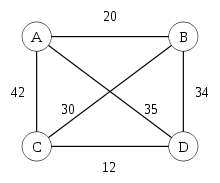
\includegraphics[scale=0.8]{images/220px-Weighted_K4.png}
	\caption{Beispiel für einen Graphen mit gewichteten Kanten und 4 Knoten als Kunden; Die Kosten sind dabei als ganze Zahlen an den Kanten angegeben; Bild: \url{www.wikipedia.org}}
	\label{fig:graph}
\end{figure}

\noindent
Um durch einen Graphen zu navigieren existieren Algorithmen, welche zum Beispiel die kürzeste Route von einem Punkt zu allen anderen im Graphen finden. 
Hierzu zählt zum Beispiel der Dijkstra-Algorithmus, der als Standardalgorithmus im Gebiet der kürzesten Routenfindung eingesetzt wird. 

\subsection{Traveling Salesman Problem (TSP)}

Das TSP oder auch unter dem Begriff \textit{Vehicel Routing Problem (VRP)} bekannt, stellt ein Grundproblem der Logistik dar. 
Bei dieser Problemstellung sollen geografische Positionen einmal angefahren werden und dies mit dem geringsten Aufwand. 
Dies lässt sich in der Abbildung \ref{fig:tsp} erkennen.
Dabei werden die größten Städte Deutschlands angefahren, der Start- und Zielpunkt sind dabei identisch. 
Dieses Problem kann mit einer Laufzeitkomplexität von $O((n-1)!/2)$ exakt gelöst werden, wobei mit zunehmender Größe des Faktors \textit{n}, die Berechnungszeit wesentlich größer wird. 
Aus diesem Grund wurden heuristische Algorithmen entwickelt, welche eine mögliche Lösung finden, aber sehr wahrscheinlich nicht die effizienteste Route. 
Heuristische Lösungen werden eingesetzt, da sie zeit- und ressourcensparender sind und dabei verwendbare Lösungen liefern \cite{wurzer2010fallbeispiele, laporte1992vehicle}. 
\begin{figure}
	\centering
	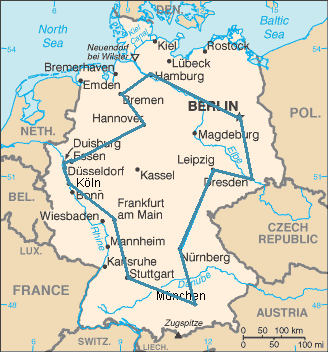
\includegraphics[scale=0.8]{images/TSP_Deutschland_3.png}
	\caption{Beispiel für eine Route durch Deutschland; Bild: \url{www.wikipedia.org}}
	\label{fig:tsp}
\end{figure}

\noindent
Weiters werden einige spezialisierte Formen des VRP kurz erklärt und beschrieben. 

\paragraph{Capacity Vehicle Routing Problem (CVRP):}

In dieser Erweiterung von VRP spielt besonders die Kapazität der Fahrzeuge eine Rolle, denn diese sollte so effizient wie möglich ausgenützt werden. 
Hierbei starten alle Fahrzeuge vom selben Depot, alle Kunden sind vorab bekannt. 
In diesem Fall besitzen alle Fahrzeuge dieselbe Kapazität, welche in der Route nicht überschritten werden darf \cite{laporte1992vehicle}. 

\noindent
Lösungsalgorithmen für CVRP:
\begin{itemize}
	\item Savings-Algorithmus: wird in Sektion \ref{savingKurz} erklärt 
	\item Der Sweep-Algorithmus verwendet ein \textit{Cluster-first} Vorgehen. 
	Hierbei werden Stopps einem Fahrzeug solange hinzugefügt, bis dessen Kapazität oder die maximale Routenlänge erreicht wird. 
	Die Zuteilung zu einem Fahrzeug wird durch Polarkoordinaten festgestellt und dessen Winkel zum aktuell ausgewählten Punkt. 
	Im Anschluss wird eine TSP Optimierung auf den erstellten Cluster an Haltepunkten ausgeführt und so eine optimierte Route generiert. 
	\item Ein \textit{Route-first} Vorgehen, wie von Beasley 1983 beschrieben, beginnt mit einer optimierten Route ohne Berücksichtigung der Nebenbedingungen. 
	Im Anschluss wird diese Route auf Fahrzeuge aufgeteilt, sodass die Nebenbedingungen eingehalten werden. 
\end{itemize} 

\paragraph{Periodic Vehicle Routing Problem (PVRP):}

PVRP stellt wie CVRP eine Erweiterung des Basisproblems dar. 
In diesem Fall sollen Kunden nicht einmal, sondern mehrmals angefahren werden. 
Dieses Problem tritt zum Beispiel bei einem Hausbau mit mehreren Betonlieferungen auf, über eine längere Zeit abhängig von der Nachfrage \cite{laporte1992vehicle}. 

\paragraph{Vehicle Routing Problem with Backhauls (VRPB):}

Das VRPB erweitert das CVRP um die Möglichkeit, Kunden nicht nur zu beliefern, sondern auch etwas entgegenzunehmen. 
Dabei entstehen zwei Teilmengen.
Kunden die beliefert werden und Kunden von welchen abgeholt werden soll. 
Im Grunde erweitert sich das Basismodell um eine Vorrangregel, bei welcher zu beliefernde Kunden bevorzugt werden. 
Ansonsten könnte der Fall eintreten, dass ein Fahrzeug keine Zusatzladung mehr aufnehmen kann \cite{wurzer2010fallbeispiele}.

\paragraph{Vehicle Routing Problem with Time Windows (VRPTW):}

Das VRPTW erweitert ebenfalls das CVRP, sodass Kunden nicht zu jeder Zeit angefahren werden können.
Dieses Problem ist aus der Praxis heraus gewachsen, denn manche Kunden und Lager sind nur zu bestimmten Zeiten anzutreffen. 
Zusätzlich könnten Straßensperren berücksichtigt werden, wie zum Beispiel eine Innenstadt mit Zustellungserlaubnis am Vormittag. 
Das Basismodell muss hierbei um Zeitintervalle erweitert werden, weiters müssen die Abfahrtszeiten vom Depot, Fahrzeiten für alle Teilstrecken und Servicezeit bei jedem Kunden vorhanden sein. 
Im Gesamten muss festgelegt werden wie optimiert werden soll, denn es besteht die Möglichkeit, dass Fahrzeuge warten müssen, bis der Kunde anzutreffen ist. 
Im Falle einer Wartezeit könnte zuerst ein anderer Kunde angefahren werden. 
Dies bedeutet, dass wahrscheinlich eine längere Strecke zurückgelegt werden muss \cite{wurzer2010fallbeispiele}. 

\noindent
Lösungsalgorithmen für VRPTW:
\begin{itemize}
	\item Savings-Algorithmus
	\item Route-first, Cluster-second (Solomen 1986)
	\item Sequentielle Einfügeheuristik (Solomon 1987)
	\item Zeitorientierte Nearest-Neighbor Heuristik 
	\item Tabu-Search
	\item Evolutionäre Algorithmen
\end{itemize} 

\paragraph{Pick-up-and-delivery Problem (PDP):}

Das PDP stellt eine zusätzliche Spezialisierung des VRP dar. 
In diesem Fall müssen Abholungen und Lieferungen in einer Route erledigt werden. 
Dabei ist die Kapazität der Fahrzeuge sehr zu berücksichtigen, da diese erst wieder zusätzliche Ladungen aufnehmen können, wenn genügend Kapazität dafür vorhanden ist. 
Außerdem muss berücksichtigt werden, dass eine Ladungsaufnahme in dieser Route später auch zugestellt wird. 
Diese Ladungen dürfen nicht als Auslieferung für eine weitere Route übernommen werden. \\

\noindent
Diese Beschreibungen stellen nur eine Teilmenge der Problemdomänen dar, weshalb für genauere Informationen Fachlektüre hinzugezogen werden sollte. 
Des Weiteren existieren Meta-Heuristische Algorithmen, welche eine geringe Laufzeit besitzen, dafür kein exaktes Ergebnis liefern, sondern nur eine Annäherung. 

\section{Lösungsverfahren}

\subsection{Exakte Verfahren}

Exakte Verfahren liefern die beste Lösung, aber nicht ohne Nachteile.  
Einer dieser Nachteile ist, dass die benötigte Zeit mit jedem weiteren Knoten im System stark ansteigt, da die zu überprüfenden Möglichkeiten  steigen. 

\paragraph{Branch-and-Cut:}	

\textit{Branch-and-Cut} vereint zwei Verfahren, welche ebenfalls im Gebiet der Logistik eingesetzt werden: Das Schnittebenenverfahren und das \textit{Branch-and-Bound} Verfahren. 
Ziel dieser ganzzahligen linearen Optimierung stellt eine lineare Zielfunktion dar, welche gesucht wird. 
Diese Funktion wird mit Hilfe von linearen Ungleichungen gesucht, welche eine Menge an Punkten umschließen. 
Durch das Schnittebenenverfahren werden weitere Ungleichungen in das System eingefügt, welche von allen zulässigen Punkten erfüllt werden. 
Durch ein weiteres Lösen des Systems muss eine neue Lösung entstehen, welche näher am gesuchten Optimum liegt.
Das \textit{Branch-and-Bound} wird im Anschluss ausgeführt, wenn keine Schnittebenen mehr gefunden werden. 
Die genauere Beschreibung dieses Algorithmus befindet sich in der Sektion \ref{Heuristik}, da dieses Verfahren in der Fachliteratur den Übergruppen \textit{exakte Verfahren} und \textit{heuristische Verfahren} zugeordnet wird. 

\subsection{Heuristik}
\label{Heuristik}

Heuristik bedeutet, mit wenig Wissen sowie mit begrenzter Zeit eine wahrscheinliche Lösung zu liefern. 
Heuristiken werden oft im Gebiet der Optimierungen eingesetzt. 
Zum exakten Lösen eines Logistik-Problems wird sehr viel Zeit und Speicher benötigt. 
Deshalb werden hier häufig Heuristiken eingesetzt. 
Ein Vorteil der Heuristik ist es, dass in kurzer Zeit gute Lösungen für schwierige Probleme gefunden können. 
Die Nachteile dieser Methoden sind aber nicht zu vernachlässigen, sie geben nämlich:
\begin{itemize}
	\item keine Garantie für die optimale Lösung;
	\item keine Garantie für eine Lösung und für die Güte einer Lösung;
\end{itemize}

\paragraph{Branch-and-Bound:}

Im Grunde wird bei diesem Algorithmus ein Baum im Sinne der Informationstechnologie aufgebaut, in welchem anhand der Möglichkeiten gesucht und verglichen wird. 
Dabei werden Schwellenwerte für die Kosten festgelegt, welche bei einer Route nicht über- und unterschritten werden dürfen.
\begin{itemize}
	\item \textit{Branchen} (Verzweigung) ist der erste Schritt in diesem Algorithmus. 
	Hierbei wird das Problem in mehrere Teilprobleme aufgeteilt und in einer Baumstruktur abgelegt. 
	\item \textit{Bounden} (Beschränkung) repräsentiert den zweiten Schritt, in welchem die Lösungsmenge beschränkt wird. 
	Dabei wird überprüft, welche Zweige suboptimal sind und als mögliche Lösungen verworfen werden. 
\end{itemize}
Eine Lösung wird verworfen, wenn das Gewicht eines \textit{1-tree} größer ist als das Gewicht einer zuvor gefundenen möglichen Lösung. 
Ein \textit{1-tree} beschreibt dabei einen Weg von der Hauptwurzel bis zu einem Endblatt. 
Diese Art der Routenfindung liefert rasch brauchbare Ergebnisse \cite{wiener2003branch}. 

\paragraph{Nearest-Neighbor (NN):}

Die NN-Heuristik stellt ein mögliches Eröffnungsverfahren dar. 
Diese liefert zwar eine Approximation der Lösungen, aber meist nicht sehr gute Resultate. 
Der Algorithmus kann dazu verwendet werden, um eine Beispiellösung zu generieren. 
Diese Lösung kann als Ausgangszustand für Verbesserungsheuristiken eingesetzt werden, welche selbst keine Grundlösung finden würden. 
Der Grundalgorithmus wählt zufällig einen Knoten aus dem System und sucht sich anhand diverser Kriterien einen weiteren Knoten, welcher als \textit{Nearest-Neigbor} bezeichnet wird. 
Von diesem ausgehend wird ein weiterer Knoten zur Route hinzugefügt, bis diese vollständig ist. 
Ein Nachteil dieses Algorithmus lässt sich am Ende erkennen, wenn die Route vollständig ist.
Start und Endpunkt liegen oft sehr weit auseinander. 
Dieses Verhalten ist meist nicht gewünscht, da eine Rundreise erwartet wird und nicht eine Route im Sinne einer Linie und einem langen Rückweg \cite{jp2010opttrans}. 

\noindent
Von diesem Algorithmus aus existieren noch einige weitere Spezialisierungen, wie zum Beispiel der \textit{Variable Neighbourhood Search} Algorithmus.
Dieser nützt den Vergleich von lokalen Optima zu globalen Optima, um effizientere Routen zu finden. 

\paragraph{Savings-Algorithmus (SA):} 
\label{savingKurz}

Der SA von Clarke und Wright gehört nicht zur Kategorie der Eröffnungsverfahren, sondern zu den Optimierungsalgorithmen. 
Bei diesem wird hauptsächlich mit einem Saving gearbeitet. 
Dieses Saving repräsentiert, wie viel gespart werden kann, wenn der Kunde \textit{B} nach dem Kunden \textit{A} angefahren wird und somit zwischen diesen Kunden nicht zum Depot zurückgekehrt werden muss. 
Dabei spielt die Berechnung des Savings aus den Kosten eine wichtige Rolle, auf welche später noch genauer eingegangen wird. 

\noindent
Der Algorithmus beruht darauf, in jedem Schritt eine Route zu vergrößern und dabei einige andere zu entfernen. 
Der grundsätzliche Ablauf sieht wie folgt aus:
\begin{enumerate}
	\item Zu Beginn müssen Werte zur Berechnung der Ersparnisse initialisiert werden, wie eine Zeit- oder Distanzmatrix. 
	In diesem Schritt wird aus jedem Knoten/Kunde eine triviale Route erstellt, bestehend aus \textit{Depot - Knoten - Depot}.
	\item Im nächsten Schritt wird jede Route mit jeder anderen Route gepaart und der Savings-Wert berechnet. 
	In diesem Schritt muss auch überprüft werden, ob die Kombinationen die Nebenbedingungen einhalten. 
	Sollte dies nicht der Fall sein, muss diese Möglichkeit verworfen werden. 
	\item Die Kombination von zwei Routen mit dem höchsten Saving, wird im Anschluss zu einer neuen Route vereint. 
	\item Nach der Kombination müssen alle Möglichkeiten entfernt werden, welche die zweite Teilroute beinhalten. 
	Zusätzlich müssen alle Teilrouten mit dem ersten Teil durch die neue Route ersetzt werden. 
	\item Infolgedessen wird bei Punkt 2 fortgesetzt, wenn sich noch Kombinationen an Routen in der Savingsliste befinden. 
	Sollte dies nicht der Fall sein, so wurde eine optimierte Route gefunden oder mehrere Teilrouten, welche nicht mehr kombiniert werden können. 
\end{enumerate}

\paragraph{Sweep-Algorithmus:}

Der Sweep-Algorithmus verwendet wie zuvor schon erwähnt ein \textit{Cluster-first} Vorgehen. 
Dieser verwendet ein geometrisches Verfahren zum Erstellen des Clusters, weshalb dieser nur in planaren Instanzen angewendet werden kann.
Jeder Kunde im System wird in einem Polarkoordinatensystem repräsentiert. 
Jeder besitzt einen Winkel und einen direkten Abstand zum zentralen Depot. 
\begin{itemize}
	\item Zu Beginn wird ein beliebiger Knoten/Kunde als erster Haltepunkt in der Route ausgewählt.
	\item Im Anschluss wird zu diesem Ausgangspunkt ein weiterer Kunde hinzugefügt und zwar dieser mit dem geringsten Winkelabstand zum letzten Punkt in der Route. 
	\item Dieser Prozess wird solange durchgeführt, bis eine Route eine maximale Anzahl an Punkten erreicht hat oder ein Fahrzeug keine Kapazität mehr zur Verfügung hat. 
	\item Damit wurde ein Cluster an Stopps für ein Fahrzeug erstellt, welcher im einem zweiten Schritt zu einer optimierten Route entwickelt werden muss. 
\end{itemize}
Somit gehört auch dieser Algorithmus zur Kategorie der Eröffnungsverfahren \cite{jp2010opttrans}. 

\subsection{Meta-Heuristiken}

Meta-Heuristik wird in der Informatik als Bezeichnung verwendet, wenn eine Lösung näherungsweise erzeugt wird. 
Diese sind nicht stark problemspezifisch orientiert, im Gegensatz zu Heuristiken. 
Diese Art von Algorithmen wird im Bereich der Logistik deshalb eingesetzt, weil sie lokalen Optima in schwereren und größeren Problemen entwischen können und eher zu einem globalen Optima tendieren oder konvergieren. 

\paragraph{Tabu-Search (TS):}

Der \textit{Tabu-Search} baut auf keiner bisher beschriebenen Methode auf. 
Im Unterschied zu anderen Algorithmen sind beim TS auch ungültige Lösungen zugelassen, welche die Nebenbedingungen verletzen. 
Es muss dafür eine Kostenfunktion existieren, mit welcher die Kosten einer Lösung festgestellt werden können. 
Für jede gefundene Lösung wird evaluiert, ob dies eine verwendbare Lösung ist oder nicht. 
Hierbei fließen die einzelnen Nebenbedingungen, mit einem hinzumultiplizierten Faktor, eine Rolle. 
So kann festgestellt werden, ob es sich um eine bessere Lösung handelt oder nicht. 
Eine Kernfunktionalität stellt die Tabu-Liste dar. 
In dieser werden Unmöglichkeiten gespeichert, welche nicht durchgeführt werden dürfen, solange sie sich in der Liste befinden. 
Zum Beispiel darf von einem Ort aus nicht nach Osten zum nächsten gefahren werden, da dieser Zug in der Iteration vorher durchgeführt worden ist. 

\noindent
Der Hauptalgorithmus besteht aus einer Hauptschleife, welche an ein Abbruchkriterium geknüpft ist. 
Zu Beginn wird dabei eine mögliche Lösung initialisiert und als aktuell beste Lösung angenommen. 
Im Anschluss werden weitere mögliche Lösungen erzeugt und die Beste daraus ausgewählt. 
Diese alternative Lösung wird mit der aktuell besten Lösung verglichen und als neue Beste definiert, wenn dies der Fall ist. 
Daraufhin wird die Tabu-Liste aktualisiert. 
Dieser Ablauf wird solange durchgeführt, bis das Abbruchkriterium eintritt.

\noindent 
Bei diesem Algorithmus wird nicht garantiert, dass eine gültige Lösung gefunden wird. 
So kann aber eine Lösung entstehen, welche weit geringere Kosten mit sich bringt als eine Lösung ohne Verletzung der Nebenbedingungen. 
Im Falle einer Applikation muss durch die Evaluierungsfunktion definiert sein, in wie weit eine Nichteinhaltung toleriert wird oder nicht \cite{jp2010opttrans}. 

\paragraph{Simulated Annealing (SA):} 

SA ist für sich im Detail kein Algorithmus, sondern bezeichnet eine Klasse von Algorithmen, welche versuchen global zu optimieren. 
Die Idee und die Bezeichnung stammen hierbei aus der Härtung von Stahl. 
In der Stahlproduktion wird dieser \textit{erwärmt} und wieder \textit{abgekühlt}, was als \textit{härten} bezeichnet wird. 
Dieser Prozess des Abkühlens führt dazu, dass sich die Teilchen wie in einer Gitterstruktur anordnen. 
Zu Beginn kann von einer stochastischen Suche gesprochen werden und zum Ende hin von einer deterministischen Suche. 
Zum Ende des Prozesses werden die Schritte immer kleiner, wie bei der Härtung kühlen dabei die letzten Temperaturen sehr langsam ab. 
Im Gesamten wird eine global optimale Konfiguration gefunden, in dem dieser Prozess simuliert wird. 
Am Anfang wird deshalb von einer stochastischen Suche gesprochen, da das System Möglichkeiten annimmt, welche zu einer Verschlechterung des Ergebnisses führen. 
Wird die sogenannte Temperatur geringer, minimiert sich die Akzeptanz für Möglichkeiten, was wiederum deterministisch ist. 
Der stochastische Anteil ermöglicht dem lokalen Minima zu entkommen und dem globalen Minima sich anzunähern. 
Der Grundalgorithmus ähnelt dabei sehr dem \textit{Tabu-Search} mit der Hauptschleife. 
Beim SA wird solange optimiert, bis das System einen erstarrten Zustand erreicht \cite{kirkpatrick1983optimization}. 

\paragraph{Ant Colony Optimierung (ACO):}

ACO repräsentiert eine Simulation von sozialen Interaktionen in der Natur.
So wurde für diesen Algorithmus das Verhalten und die Interaktionen von Ameisen, Bienen und weiteren Insekten analysiert. 
Jedes Individuum dieser Insekten erledigt eine eigene Aufgabe, unabhängig von anderen in der Kolonie. 
Ein funktionierendes System kommt dadurch zustande, dass die Arbeiten jedes einzelnen Individuums auf den Arbeiten eines anderen aufbauen oder mit anderen verbunden sind.
Durch die Kooperation in der Kolonie, entsteht die Möglichkeit, komplexe Probleme zu lösen und Überlebensstrategien auszuführen \cite{mucherino2015ant, abraham2006swarm}. 

\noindent
Damit dieser Algorithmus eingesetzt werden kann, müssen einige Grundvoraussetzungen erfüllt sein:
\begin{itemize}
	\item Eine Strategie zum Überprüfen einer gültigen Lösung, damit nur solche akzeptiert werden;
	\item Eine heuristische Funktion $\eta$ zum Messen der Qualitäten der Teile, welche sich noch nicht in der Teillösung befinden;
	\item Eine Funktion zum Aktualisieren der Pheromone $\tau$, welche die Wertigkeit der Kanten repräsentiert; 
	\item Eine Funktion $\phi$, welche auf der heuristischen Funktion $\eta$ und den Pheromonen aus $\tau$ basiert und iterativ mögliche Lösungen konstruiert;  
\end{itemize}

\noindent
Der grobe Ablauf des Grundalgorithmus: 
\begin{itemize}
	\item Zu Beginn wird die Ameise an einem Startpunkt ausgesetzt;
	\item Diese besitzt nun die Möglichkeit sich mit einer bestimmte Anzahl von Zügen durch das Netzwerk zu bewegen unter Berücksichtigung der Funktion $\phi$; dabei wird eine Tabu-Liste für diese Ameise erstellt; 
	\item Im Anschluss wird die Tour der Ameise bewertet und
	die Pheromone der Kanten berechnet; eine weitere Ameise wird ausgesetzt bis die maximal Anzahl der Ameisen erreicht ist;
	\item Nachdem alle Ameisen einmal im Netzwerk waren, werden alle Pheromone an den Kanten aktualisiert; 
	\item Diese entstandene Lösung wird nun mit der letzten verglichen und ein weiterer Durchlauf wird unter Berücksichtigung eines Abbruchkriteriums mit den neuen Pheromonen eingeleitet; 
\end{itemize}

\paragraph{Evolutionäre Algorithmen (EA):}

EA sind wie SA kein Algorithmus, sondern ein Überbegriff für eine Klasse von Algorithmen und Methoden. 
Das Prinzip dieser Algorithmen beruht auf dem Vorgang einer biologischen Evolution. 
Die Natur einer biologischen Evolution ist es, sich zu verbessern und zu überleben, was äquivalent zu einem Optimierungsprozess ist. 
In der Natur sind die Vorgänge der Optimierung bei einem Menschen sehr langsam und für ein einzelnes Individuum nicht wahrnehmbar. 
Dabei muss sich jede Generation aufs Neue behaupten und beweisen, dass sie mit der aktuellen Umgebung besser zurechtkommt. 
Diese Selektion geschieht ganz nach \textit{Charles Darwins} Worten \textit{survival of the fittest}, sodass der Angepassteste/Fitteste sich am stärksten verbreitet beziehungsweise vermehrt. 
Die Veränderungen entstehen dabei durch einfache Fortpflanzung im Sinne einer Rekombination und durch Mutationen. 
So wird bei der Mutation nur ein Individuum benötigt, welches verändert wird und bei der Rekombination zwei. 

\noindent
Ein EA besitzt genau solche Eigenschaften und versucht hier die Natur nachzuahmen. 
Im Sinne eines Algorithmus werden die Rekombination und Mutation schneller durchgeführt, sodass immer Mengen an potentiellen Lösungen zur Verfügung stehen. 
Alle Lösungen werden evaluiert und ihre Fitness bestimmt. 
Unbrauchbare Lösungen werden aussortiert, wenn sie nicht fit genug sind, bis eine geeignete Lösung gefunden wurde oder ein Abbruchkriterium wirksam wird \cite{isl2008ea, beyer2001evolution}. 

\noindent
Der grundsätzliche Ablauf sieht wie folgt aus:
\begin{enumerate}
	\item Zu Beginn muss eine Beispiellösung initialisiert und bewertet werden, um einen Ausgangszustand zu erlangen; 
	\item Im Anschluss wird eine Selektion durchgeführt; 
	\item Die Selektierten werden rekombiniert und so Nachkommen erzeugt; 
	\item Auf die gesamte Menge an Lösungen wird eine Mutation angewendet; 
	\item Zum Abschluss werden alle Lösungen bewertet und ihre Fitness wird festgestellt;
	\item Sollte kein Abbruchkriterium erfüllt sein, so wird ab Punkt 2 wieder fortgesetzt; 
\end{enumerate}

\noindent
In diesem Kapitel wurden grundlegende Eigenschaften in der Logistik erklärt und Problemgebiete aufgezeigt. 
Es wurden einige Lösungsansätze beschrieben, um deren Grundalgorithmus zu verstehen. 
Im nächsten Kapitel wird auf Kostenfunktionen eingegangen und Probleme darin aufgezeigt. 
\chapter{Kostenberechnung}
\label{Kostenberechnung}

Die Kostenfunktion stellt in jedem VRP und dessen Ablegern eine Kernkomponente dar. 
Diese muss an das Problem angepasst werden und ist somit problem- und zielspezifisch. 
Mit dieser Funktion wird definiert wie und was optimiert werden soll. 
Zum Beispiel kann diese so ausgelegt sein, dass die Strecke oder Fahrzeit minimal sein soll oder beides gemeinsam. 
Im weiteren Verlauf dieses Kapitels wird auf einige Eigenschaften der Kostenfunktion für den Savings-Algorithmus eingegangen.  

\section{Distanz-Basierend}

Rein auf Distanz-Basierende-Kostenfunktionen bringen meist nicht das gewünschte Ergebnis zu Tage. 
Dies lässt sich auf die Einschränkung der vorhandenen Daten zurückführen. 
Alle Ergebnisse basieren dabei rein auf den Distanzen, welche gefahren werden. 
In diesem Fall könnte ein Kunde einige wenige Kilometer entfernt sein, direkt aber nur über einen Feldweg. 
Dies würde zu einer kurzen Distanz führen ohne die Beschaffenheit der Strecke und der dabei benötigten Zeit zu berücksichtigen. 
Sollte trotzdem nur die Distanz zur Verfügung stehen, so ist dies besser als überhaupt keine Informationen zu haben. 

\noindent
Die Berechnung für die Ersparnis im SA ist in der Gleichung \ref{eq:savingbase} zu finden. 
Dabei stellen die Punkte \textit{A} und \textit{B} zwei Kunden dar und \textit{DE} das Depot, von welchem aus losgefahren wird. 
Die Variable \textit{dis} repräsentiert die Distanzmatrix, welche alle Distanzen zwischen den Punkten beinhaltet. 
Die Ersparnis ist hierbei definiert als das, was eingespart wird, wenn zwischen Kunde \textit{A} und \textit{B} nicht zum Depot zurückgekehrt, sondern direkt von \textit{A} nach \textit{B} gefahren wird \cite{clarke1964scheduling}. 
\begin{equation}
sav_{a,b} := dis_{a,z} + dis_{z,b} - dis_{a,b}
\label{eq:savingbase}
\end{equation}

\noindent
In der Abbildung \ref{fig:simpleNetwork} ist ein einfaches Netzwerk mit Kunden und einem Depot abgebildet. 
Die Abkürzung \textit{AB} steht in diesem Beispiel für Autobahn, \textit{LS} für Landstraße und \textit{FW} für Feldweg. 
Wie in dieser Abbildung festgestellt werden kann, existieren zwei Kanten mit einem Feldweg und eine mit einer Autobahn. 
An diesem Beispiel lässt sich erkennen, dass die Beschaffenheit des Fahrwegs ignoriert und vernachlässigt wird. 
In Tabelle \ref{tab:distSavings} befinden sich die Ergebnisse der Ersparnisse zu Beginn des Savings-Algorithmus nach der Initialisierung. 
Im Gesamten lässt sich hier erkennen, dass lange Strecken bevorzugt werden. 
In diesem Fall würden zuerst die Routen \textit{A - B} oder \textit{D - E} zusammengefügt werden, abhängig von der Sortierung der Savings-Liste. 
\begin{figure}
\centering
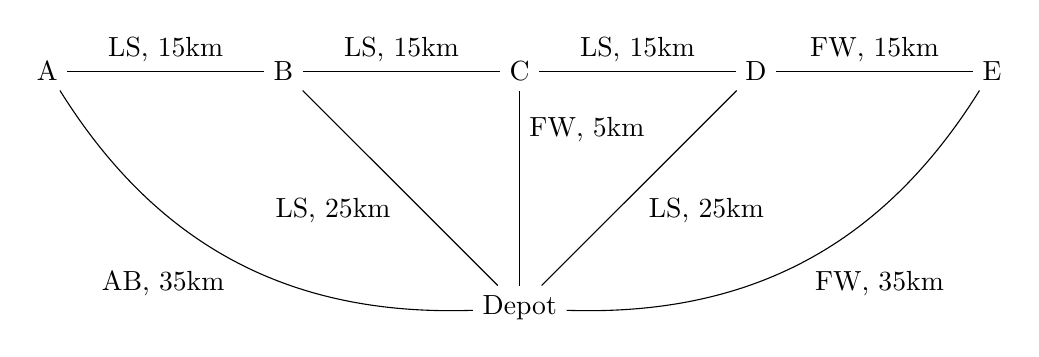
\begin{tikzpicture}[auto, node distance=3cm]
	%\tikzstyle{every node}=[draw,shape=circle];
	
	\node (a) {A};
	
	\node (b) [right of=a] {B};
	
	\node (c) [right of=b] {C};
	
	\node (d) [right of=c] {D};
	
	\node (e) [right of=d] {E};
	
	\node (de) [below of=c] {Depot};
	
	\path 	(de) 	edge [bend left] node {AB, 35km} (a)
					edge node {LS, 25km} (b)
			 		edge node [right, pos=0.8] {FW, 5km} (c)
			 		edge node [below right] {LS, 25km} (d)
			 		edge [bend right] node [below right] {FW, 35km} (e)
			(a)		edge node {LS, 15km} (b)
			(c) 	edge node [above] {LS, 15km} (b)
			(d)		edge node [above] {LS, 15km} (c)
			(d)		edge node {FW, 15km} (e);
\end{tikzpicture}

	\caption{Ein einfaches Netzwerk mit $4$ Kunden und einem Depot}
	\label{fig:simpleNetwork}
\end{figure}
\begin{table}[htb]%[ht!]
\centering% NICHT \begin{center}
\begin{tabular}{p{3cm}|p{4cm}}
%\hline 
Route & Ersparnis \\ 
\hline 
A $\leftrightarrow$ B & $35 + 25 - 15 = 45$ \\ 
%\hline 
B $\leftrightarrow$ C & $25 + 5 - 15 = 15$ \\ 
%\hline 
C $\leftrightarrow$ D & $5 + 25 - 15 = 15$ \\ 
%\hline 
D $\leftrightarrow$ E & $25 + 35 - 15 = 45$ \\ 
%\hline 
\end{tabular} 
\caption{Aufschlüsselung der Ersparnisse anhand der Teilrouten zu Beginn der Optimierung}
\label{tab:distSavings}
\end{table}

\noindent
An diesem Beispiel lässt sich erkennen, dass die Beschaffenheit einer Straße ignoriert wird. 
Für den Algorithmus sieht dies so aus, als ob dies eine gute Kombination wäre.
Im Grund stimmt dies, zumal die Ersparnis größer ist. 

\section{Zeit-Basierend}

Zeit-Basierende-Kostenfunktionen beinhalten einen Vorteil gegenüber der Distanz-Basierten-Version, aber bergen auch Probleme. 
Der Vorteil der Zeitinformation liegt darin, dass die Beschaffenheit der Strecke versteckt mit einfließt. 
So wird auf einer Strecke mit Autobahn weniger Zeit benötigt, als auf derselben Distanz, aber mit Feldweg als Beschaffenheit. 

\noindent
Die Berechnung für die Ersparnis im Savings-Algorithmus ist in der Gleichung \ref{eq:savingbasezeit} zu finden. 
Dabei ist diese identisch mit der Gleichung aus \ref{eq:savingbase} mit dem Unterschied, dass hier eine Zeitmatrix \textit{time} verwendet wird. 
\begin{equation}
sav_{a,b} := time_{a,z} + time_{z,b} - time_{a,b}
\label{eq:savingbasezeit}
\end{equation}

\noindent
In Abbildung \ref{fig:simpleNetworkTime} befindet sich das gleiche Netzwerk aus \ref{fig:simpleNetwork}, aber mit Zeiten an den Kanten. 
Die Abkürzung \textit{AB} steht für Autobahn mit $130\,km/h$, \textit{LS} für Landstraße mit $100\,km/h$ und \textit{FW} für Feldweg mit $10\,km/h$. 
In der Tabelle \ref{tab:distSavingsZeit} befinden sich die Ergebnisse der Ersparnisse zu Beginn des Savings-Algorithmus nach der Initialisierung.
Erkennbar ist hier, dass nicht die Strecke mit der Autobahn bevorzugt wird, sondern der langsame Feldweg. 
Dieses Verhalten führt unweigerlich dazu, dass der Feldweg als erste Kombination verwendet wird. 
\begin{figure}
\centering
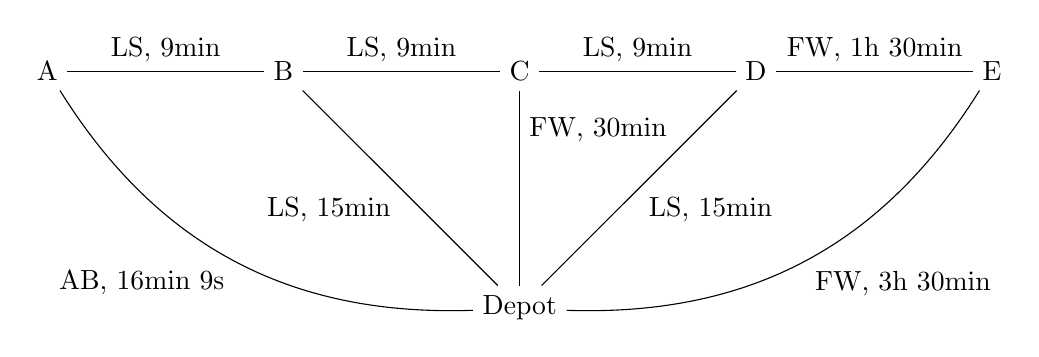
\begin{tikzpicture}[auto, node distance=3cm]
	%\tikzstyle{every node}=[draw,shape=circle];
	
	\node (a) {A};
	
	\node (b) [right of=a] {B};
	
	\node (c) [right of=b] {C};
	
	\node (d) [right of=c] {D};
	
	\node (e) [right of=d] {E};
	
	\node (de) [below of=c] {Depot};
	
%	\path 	(de) 	edge node {AB, 16min 9s} (a)
%					edge [bend left] node {LS, 15min} (b)
%			 		edge node {FW, 30min} (c)
%			 		edge [bend right] node {LS, 15min} (d)
%			 		edge node {FW, 3h 30min} (e)
%			(a)		edge [bend right] node {LS, 9min} (b)
%			(c) 	edge [bend right] node {LS, 9min} (b)
%			(d)		edge [bend right] node {LS, 9min} (c)
%			(d)		edge [bend right] node {FW, 9min} (e);
			
	\path 	(de) 	edge [bend left] node {AB, 16min 9s} (a)
					edge node {LS, 15min} (b)
			 		edge node [right, pos=0.8] {FW, 30min} (c)
			 		edge node [below right] {LS, 15min} (d)
			 		edge [bend right] node [below right] {FW, 3h 30min} (e)
			(a)		edge node {LS, 9min} (b)
			(c) 	edge node [above] {LS, 9min} (b)
			(d)		edge node [above] {LS, 9min} (c)
			(d)		edge node {FW, 1h 30min} (e);
\end{tikzpicture}

	\caption{Derselbe Graph aus \ref{fig:simpleNetwork} mit $4$ Kunden und einem Depot mit den benötigten Zeiten}
	\label{fig:simpleNetworkTime}
\end{figure}
\begin{table}[htb]%[ht!]
\centering% NICHT \begin{center}
\begin{tabular}{p{3cm}|p{4cm}}
%\hline 
Route & Ersparnis \\ 
\hline 
A $\leftrightarrow$ B & $16,15 + 15 - 9 = 22,15$ \\ 
%\hline 
B $\leftrightarrow$ C & $15 + 30 - 9 = 36$ \\ 
%\hline 
C $\leftrightarrow$ D & $30 + 15 - 9 = 36$ \\ 
%\hline 
D $\leftrightarrow$ E & $15 + 210 - 90 = 135$ \\ 
%\hline 
\end{tabular} 
\caption{Aufschlüsselung der Ersparnisse anhand der Teilrouten zu Beginn der Optimierung mit den benötigten Zeiten als Basis}
\label{tab:distSavingsZeit}
\end{table}

\section{Distanz-Zeit-Basierend}
\label{sec:disZeitBase}

Eine Kostenberechnung mit Distanz- und Zeitwerten bietet die Möglichkeit, die Beschaffenheit der Strecke zu berücksichtigen und so zum Beispiel Feldwege zu ignorieren. 
Diese Daten erzeugen ein Problem. 
Es wirft die Frage auf, wie die Distanzen und die Zeiten in eine Relation gesetzt werden sollen. 
Einfaches Addieren würde dazu führen, dass eine Strecke von $45\,km$ mit einer Geschwindigkeit von $10\,km/h$ zu einer ungewollt hohen Ersparnis führen würde. 
Damit dieses Verhalten nicht auftritt, muss ein Wert durch den anderen dividiert werden. 

\noindent
Eine für diesen Fall akzeptable Verhältnisrechnung wäre eine Division aus der Strecke in Metern und der Zeit in Minuten. 
In Tabelle \ref{tab:disTimeValues} sind hierzu die Wertigkeiten der Kanten aus den Abbildungen \ref{fig:simpleNetwork} und \ref{fig:simpleNetworkTime} zu finden. 
An diesem Beispiel lässt sich erkennen, dass die Kante vom \textit{Depot} zum Knoten \textit{A} mit $2786,37$ besser bewertet wird, im Gegensatz zu der Kante vom \textit{Depot} zum Knoten \textit{E}. 
Im Grunde ist so ein Verhalten das Gewünschte, denn eine Strecke mit einer schlechten Streckenbeschaffenheit wird schwächer bewertet. 
\begin{table}[htb]%[ht!]
\centering% NICHT \begin{center}
\begin{tabular}{p{5cm}|p{5cm}}
%\hline 
Kante & Wertigkeit \\ 
\hline 
A $\leftrightarrow$ B, B $\leftrightarrow$ C, C $\leftrightarrow$ D & $15000m / 9min = 1666,67$ \\ 
%\hline 
D $\leftrightarrow$ E & $15000m / 90min = 166,67$ \\ 
%\hline
Depot $\leftrightarrow$ A & $45000m / 16,15min = 2786,37$ \\ 
%\hline 
Depot $\leftrightarrow$ B, Depot $\leftrightarrow$ D & $25000m / 15min = 1666,67$ \\ 
%\hline 
Depot $\leftrightarrow$ C & $5000m / 30min = 166,679$ \\ 
%\hline 
Depot $\leftrightarrow$ E & $45000m / 210min = 214,29$ \\
%\hline
\end{tabular} 
\caption{Aufschlüsselung der Kantenwertigkeit anhand der Strecke und der dafür benötigten Zeit}
\label{tab:disTimeValues}
\end{table}
Für die weitere Savingsberechnung kann die Basisberechnung verwendet werden, mit der berechneten Distanz-Zeit-Matrix. 
Diese Matrix beinhaltet dabei die Werte wie zuvor beschrieben. 

\noindent
Basierend auf den in der Tabelle \ref{tab:disTimeValues} berechneten Kantenwertigkeiten beinhaltet die Tabelle \ref{tab:savingsDZ} die daraus resultierenden Ersparnisse. 
Dafür wird derselbe Graph aus \ref{fig:simpleNetwork} mit den neuen Kantenwertigkeiten verwendet. 
An diesem Beispiel lässt sich erkennen, dass die Autobahn vom \textit{Depot} zum Knoten \textit{A} bevorzugt wird. 
\begin{table}[htb]%[ht!]
\centering% NICHT \begin{center}
\begin{tabular}{p{3cm}|p{7cm}}
%\hline 
Route & Ersparnis \\ 
\hline 
A $\leftrightarrow$ B & $2786,37 + 1666,67 - 1666,67 = 2786,37$ \\ 
%\hline 
B $\leftrightarrow$ C & $1666,67 + 166,67 - 1666,67 = 166,67$ \\ 
%\hline 
C $\leftrightarrow$ D & $166,67 + 1666,67 - 1666,67 = 166,67$ \\ 
%\hline 
D $\leftrightarrow$ E & $1666,67 + 214,29 - 166,67 = 1724,29$ \\ 
%\hline 
\end{tabular} 
\caption{Ersparnisse für die Kombinationen mit den berechneten Werten aus Distanz und Zeit}
\label{tab:savingsDZ}
\end{table}

\noindent
Die Findung der passenden Kostenberechnung stellt den Entwickler des Algorithmus vor ein größeres Problem, als die Implementierung des grundsätzlichen Algorithmus. 
So sollten mehrere Überlegungen festgehalten und getestet werden. 
So kann das Verhalten festgestellt werden und auch in welche Richtung optimiert wird. 
Das Überprüfen und Testen kann einfach in einem Script mit einem Graph aus der Praxis erfolgen, bei welchem die optimale Route bekannt ist. 
Auf diese Art kann sichtbar gemacht werden, wie gut der Algorithmus und dessen Kostenfunktion optimieren und Lösungen finden. 

%\section{Justierung \& Anpassung}

%\paragraph{Hyperparameter}

%\paragraph{Algorithmische Anpassung}

%\paragraph{Auswirkung}


\chapter{Problemgebiete}

\section{Kostenberechnung}

Die Kostenberechnung und somit im Falle des SA die Savings-Funktion stellt den Entwickler dieser Funktion vor eine größere Herausforderung. 
Dabei können Fehler entstehen, die meist nur sehr schwer zu finden sind und zwar nur, wenn ein gesamter Prozess durchgesteppt wird. 
Hier empfiehlt es sich eine Liste der zeitlichen Werte zu notieren, um im Nachhinein die Historie des Ablaufes noch einmal aufarbeiten zu können. 

\noindent
Wie in Sektion \ref{sec:disZeitBase} erkennbar ist, führt eine Verhältnismatrix dazu, dass unterschiedliche lange Strecken vom selben Typ zum selben Wert führen. 
Das Ergebnis führt dazu, dass die Knoten, welche an eine Autobahn angebunden sind, zu Beginn verknüpft werden. 
Im Anschluss folgt die nächsten Klasse. 
Das Ergebnis wirkt hier auf den ersten Blick zufriedenstellend, aber nicht, wenn dies weiter verfolgt wird. 
Eine Abhilfe schafft dabei das Einbeziehen der Distanz in die Berechnung. 
Wie in der Gleichung \ref{eq:savingbasezeitext} festgehalten, kann auf diese Weise eine Differenzierung erreicht werden. 
\begin{equation}
kost_{a,b} := dis_{a,b} * (\frac{dis_{a,b}}{time_{a,b}})
\label{eq:savingbasezeitext}
\end{equation}
Diese Gleichung ermöglicht es Kanten mit großen Werten und unbrauchbaren Eigenschaften diese zu neutralisieren. 

\section{Nebenbedingung}

Nebenbedingungen bieten die Möglichkeit, die konkrete Problemstellung in den Algorithmus einfließen zu lassen. 
Bei diesen muss beachtet werden, dass diese immer überprüft werden. 
Sollte eine Verletzung eintreten, muss zusätzlich entschieden werden, ob diese Möglichkeit verworfen werden soll oder doch toleriert wird. 
Im Falle einer Tolerierung kann zusätzlich mit Strafen gearbeitet werden, sodass eine solche Möglichkeit an Gewichtung verliert. 

\paragraph{Time Windows (Zeitfenster):} 

Mit der Verwendung von Zeitfenstern besteht die Erweiterung der Knoten um Zeitbereiche, in welchen ein Kunde anzutreffen ist. 
Für diesen Fall müssen alle Knoten mit dieser Information ausgestattet werden oder eine Standardzeit angenommen werden. 
Bei der Verwendung in einem Savings-Algorithmus muss bei jeder Berechnung der neuen Ersparnisse überprüft werden, ob diese Nebenbedingung eingehalten wird. 
Der Grundalgorithmus geht anlässlich einer Verletzung von einer scharfen Nichteinhaltung aus. 
Dies führt zur Entfernung einiger Möglichkeiten. 
Eine weitere Möglichkeit bietet das Herabstufen einer solchen Möglichkeit, was zu einer sogenannten weichen Nebenbedingung führt. 

\noindent
Es kann definitiv die Aussage getroffen werden, dass Routing-Optimierungen kein triviales Problem darstellen. 
In diesem Sinne gehören sie auch zu der Kategorie \textit{NP-vollständig}. 
Dies bedeutet, dass sie sich nichtdeterministisch in Polynomialzeit lösen lassen. 
So gibt es viele Möglichkeiten, um das Problem zu lösen, aber nicht ohne entsprechenden zeitlichen Aufwand. 
Die Polynomialzeit bildet dabei eine Grenze zwischen dem Bereich des \textit{praktisch lösbaren} sowie \textit{praktisch nicht lösbaren}. \newline

\noindent
Im folgenden Kapitel wird ein Beispiel mit dem Savings-Algorithmus aufgearbeitet. 
Anhand dessen wird die Auswirkung der letzten Kosten/Savings-Funktion mit der Gleichung \ref{eq:savingbasezeitext} genauer überprüft. 
\chapter{Logistik mit Zeitfenster}
\label{Logistik mit Zeitfenster}

\section{Saving mit Zeitfenster in Python}

Dieses Beispiel stellt eine vereinfachte Welt dar, welche mit $5$ Knoten/Kunden und $1$ Depot ausgestattet ist. 
Das gesamte Netzwerk wurde nicht voll vernetzt, wie in Abbildung \ref{fig:exampleNetzwerk} ersichtlich ist. 
\begin{figure}
\centering
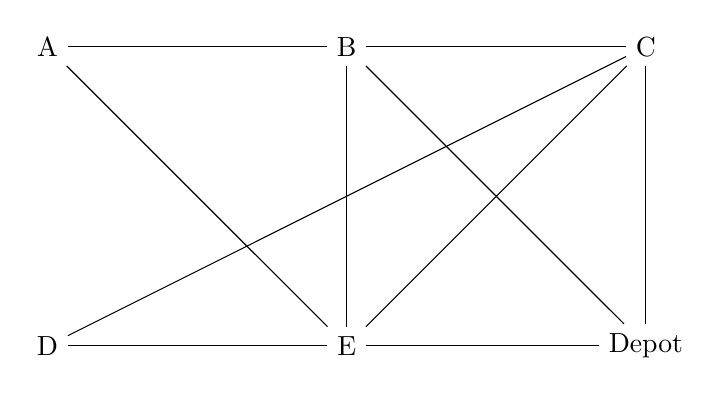
\begin{tikzpicture}[auto, node distance=3.8cm]
	%\tikzstyle{every node}=[draw,shape=circle];
	
	\node (a) {A};
	
	\node (b) [right of=a] {B};
	
	\node (c) [right of=b] {C};
	
	\node (d) [below of=a] {D};
	
	\node (e) [right of=d] {E};
	
	\node (de) [right of=e] {Depot};
	
	\path 	(de) 	edge node {} (b)
					edge node {} (c)
			 		edge node {} (e)
			(a)		edge node {} (b)
					edge node {} (e)
			(b)		edge node {} (c)
					edge node {} (e)
			(c) 	edge node {} (d)
					edge node {} (e)
			(d)		edge node {} (e);
\end{tikzpicture}

	\caption{Beispiel Graph mit $5$ Knoten/Kunden und $1$ Depot}
	\label{fig:exampleNetzwerk}
\end{figure}
Aus diesem Grund muss der Knoten \textit{D} von \textit{A} oder \textit{B} aus über \textit{E} angefahren werden. 
Dies gilt auch für die Strecke vom Depot aus. 
Die Zeit- und Distanzmatrix sind in diesem Beispiel vollständig. 
So beinhalten sie auch die kombinierte Strecke von \textit{A $\rightarrow$ E $\rightarrow$ D} mit den aufsummierten Kosten. 
In Tabelle \ref{tab:edgeValues} sind alle benötigten Werte des Graphen \ref{fig:exampleNetzwerk} aufgeschlüsselt. 
Hierbei muss beachtet werden, dass die Zeit in Minuten und Sekunden angegeben ist. 
\begin{table}[htb]%[ht!]
\centering% NICHT \begin{center}
\begin{tabular}{c|c|c|c}
%\hline 
Kante & km/h & km & Zeit (mm:ss) \\ 
\hline 
A $\leftrightarrow$ B & 80 & 10 & 07:30 \\ 
%\hline 
A $\leftrightarrow$ E & 100 & 14,14 & 08:29 \\ 
%\hline 
B $\leftrightarrow$ C & 90 & 10 & 06:40 \\ 
%\hline 
B $\leftrightarrow$ E & 110 & 10 & 05:27 \\ 
%\hline 
B $\leftrightarrow$ DE & 100 & 14,14 & 08:29 \\ 
%\hline 
C $\leftrightarrow$ D & 130 & 22,36 & 10:19 \\ 
%\hline 
C $\leftrightarrow$ E & 70 & 14,14 & 12:07 \\ 
%\hline 
C $\leftrightarrow$ DE & 100 & 10 & 06:00 \\ 
%\hline 
D $\leftrightarrow$ E & 90 & 10 & 06:40 \\ 
%\hline 
E $\leftrightarrow$ DE & 100 & 10 & 06:00 \\ 
%\hline 
\end{tabular} 
\caption{Aufschlüsselung der Distanzen, Durchschnittsgeschwindigkeiten und der benötigten Zeiten}
\label{tab:edgeValues}
\end{table}
Das Beispiel beinhaltet den gesamten Algorithmus \ref{list:algo}, welcher mit der Skriptsprache Python implementiert ist. 
Wie in einer Sektion zuvor schon beschrieben muss mit der Initialisierung begonnen werden. 
Hierzu müssen die Kostenmatrix sowie die trivialen Routen erstellt werden. 
Bei der Distanzmatrix ist zu beachten, dass diese in Kilometern beschrieben ist und intern auf Meter umgerechnet wird. 
Des Weiteren beinhaltet die Zeitmatrix die Zeiten bereits in Sekunden. 
In dieser Implementierung des Algorithmus werden alle Zeiten in Sekunden gerechnet inklusive der Wartezeiten. 

\noindent
Eine triviale Route beinhaltet nur einen Knoten, sodass die Strecke \textit{Depot $\rightarrow$ Knoten/Kunde $\rightarrow$ Depot} abgebildet wird. 
Weiters werden die möglichen Kombinationen erstellt und deren Ersparnis berechnet. 
Bei der Berechnung des Savings-Wertes muss die Nebenbedingung der Zeitfenster überprüft werden. 
Dieser erste Schritt erstreckt sich von Zeile $23$ bis Zeile $70$. 

\noindent
Im zweiten Schritt werden Routen kombiniert, bis keine Kombinationen mehr durchführbar sind. 
Dabei müssen nach der Kombination zweier Routen alle Einträge aus der Saving-Liste aktualisiert werden.
Zu diesen Aktualisierungsaufgaben zählen:
\begin{itemize}
	\item Entfernen aller Kombinationen, welche die zweite Route als Teil beinhalten;
	\item Ersetzen aller Routen in Kombinationen, welche die erste Route als Teil beinhalten;
\end{itemize}
Im Abschluss des zweiten Teils müssen die Ersparnisse mit überarbeiteten Routen neu berechnet und dabei die Zeitfenster geprüft werden. 
\lstinputlisting[language=Python,caption={Basis Implementierung des Saving-Algorithmus mit Zeitfenster},label=list:algo]{routing/routing.py}

\section{Ergebnis}

Gesamtheitlich kann festgestellt werden, dass eine grundsätzlich optimierte Route gefunden wurde. 
Trotzdem sieht es danach aus, als ob es noch bessere Routen geben müsste, wie im Ergebnis \ref{list:result} ersichtlich. 
Dabei muss wiederholt werden, dass es sich bei diesem Algorithmus um eine heuristische Lösung handelt. 
\lstinputlisting[caption={Ergebnis des Beispiels}, label=list:result, firstline=195]{routing/result.txt}

\noindent
Die Route \textit{Depot $\rightarrow$ E $\rightarrow$ D $\rightarrow$ A $\rightarrow$ B $\rightarrow$ C $\rightarrow$ Depot} spiegelt zusätzlich eine Eigenheit des Savings-Algorithmus wieder. 
Dazu muss die Historie genauer betrachtet werden. 
Wie im Listing \ref{list:firstMerge} zu erkennen ist, werden in der ersten Vereinigung die Routen mit den Knoten \textit{A} und \textit{B} kombiniert. 
Der Grund liegt in der Ersparnis, da Knoten, die weiter vom Depot entfernt sind und nahe beieinander liegen, einen hohen Wert erlangen. 
\lstinputlisting[caption={Erste Kombination von zwei Teilrouten}, label=list:firstMerge, firstline=69, lastline=78]{routing/result.txt}
Im Vergleich dazu bekommt die Vereinigung \textit{C $\leftrightarrow$ D} nur auf einen sehr niedrigen Wert. 
Dies kommt mit der großen Entfernung zwischen den Punkten zustande und der geringeren Entfernung zum Depot. 

\noindent
In einem direkten Vergleich der generierten Tour und einer manuell zusammengestellten Tour lässt sich feststellen, dass es eine bessere Route gibt. 
In der Tabelle \ref{tab:genTour} befinden sich die Zeit- und Distanzkosten der generierten Tour. 
\begin{table}[htb]%[ht!]
\centering% NICHT \begin{center}
\begin{tabular}{c|c|c|c|c|c|c|c}
%\hline 
 & E & D & A & B & C & DE & Summe\\ 
\hline 
Zeit & 360 & 400 & 400 + 509 & 450 & 400 & 360 & 2879 s \\
%\hline 
Distanz & 10 & 10 & 10 + 14,14 & 10 & 10 & 10 & 74,14 km \\
%\hline 
\end{tabular} 
\caption{Benötigte Zeit und Strecke der generierten Tour}
\label{tab:genTour}
\end{table}
Die Tabelle \ref{tab:manTour} beinhaltet die Zeit- und Distanzkosten der manuellen erstellten Tour.
\begin{table}[htb]%[ht!]
\centering% NICHT \begin{center}
\begin{tabular}{c|c|c|c|c|c|c|c}
%\hline 
 & C & D & E & A & B & DE & Summe\\ 
\hline 
Zeit & 360 & 619 & 400 & 509 & 450 & 509 & 2847 s \\
%\hline 
Distanz & 10 & 22,36 & 10 & 14,14 & 10 & 14,14 & 60,64 km \\
%\hline 
\end{tabular} 
\caption{Benötigte Zeit und Strecke der manuellen Tour}
\label{tab:manTour}
\end{table}
Im Vergleich lässt sich erkennen, dass die Kante \textit{C $\leftrightarrow$ D} mehr Zeit und Distanz mit sich bringt. 
Dafür wird die Kante \textit{D $\leftrightarrow$ E} nicht mehrfach benötigt. 
Der zeitliche Unterschied liegt bei $32$ Sekunden ohne Berücksichtigung der Wartezeiten. 
In Bezug auf den realen Straßenverkehr, kann dieser Wert vernachlässigt werden. 
Die berechnete Kostenmatrix führt in diesem Fall dazu, dass die Strecke und die Zeit optimiert werden. 
Sollte aber die Distanz minimiert werden, so müsste eine Distanzmatrix als Kostenmatrix verwendet werden. 
Eine andere Möglichkeit wäre die Berechnung der Kosten abzuändern, sodass sich die Distanzen stärker widerspiegeln. 
%\lstinputlisting[language=Python,caption={Grundklassen mit Knoten/Kunden, Routen sowie Saving-Repräsentierung},label=list:domOject]{routing/route.py}


\chapter{Zusammenfassung}
\label{Zusammenfassung}

%Routing allgegenwärtig (navis, Google maps), aber einfache point-to-point mit Zwischenstopp in fixer Reihenfolge. Es gibt aber mehr Fragestellungen @routing und entsprechend Algorithmen. Im Rahmen der Arbeit mehr routing-Algorithmen genauer kennengelernt, speziell mit Einsatz in Logistik, die heute unser leben prägt. Kurz welche algos und technische limits
Routing in der Logistik bietet die Möglichkeit effizienter Auslieferungen zu erledigen. 
Dabei existieren allgegenwärtig Navigationssysteme wie Google Maps. 
Diese Lösungen liefern meist nur die Möglichkeit einfache \textit{point-to-point} Optimierungen durchzuführen. 
Diese Konsumentenlösungen verwenden ohne Internetzugang nur Offline-Daten ohne aktuelle Verkehrslagen zu berücksichtigen. 
Im Falle von Belieferungen wird eine höhere Abstraktion benötigt.
So muss nicht nur die Strecke zwischen den Haltepunkten optimiert werden, sondern auch die Reihenfolge dieser. 
Dies führt somit von \textit{point-to-point} Optimierungen, wie der Dijkstra-Algorithmus, zu Knoten/Kunden Optimierungen, wie dem \textit{Tabu-Search}. 

\noindent
Im Rahmen der Arbeit wurden einige Problemstellungen der Logistik aufgezeigt. 
Es wurden auch mögliche Lösungsansätze für solche Probleme gezeigt und beschrieben. 
Der Savings-Algorithmus mit seinen Eigenheiten wurde zudem genauer beschrieben. 
Des Weiteren stellen Kostenfunktionen eine zentrale Komponente in Routing-Algorithmen dar. 
Durch diese wird definiert, wie und nach was optimiert wird. 

\noindent
Der Einsatz von Optimierungen in der Logistik benötigt spezielle Algorithmen. 
Die Komplexität solcher Routing-Probleme stellt eine besondere Herausforderung dar. 
So kann in begrenzter Zeit nicht einfach das Optimum gefunden werden.
Eine Ausnahme besteht, wenn die Anzahl an Stopps so gering ist, dass alle Kombinationen getestet werden können. 
Aus dieser zeitlichen Einschränkung heraus werden meistens heuristische und meta-heuristische Lösungen verwendet. 
Somit werden Routing-Probleme, wie das \textit{Traveling Salesman Problem}, die Menschheit noch weiter beschäftigen. 

%%%----------------------------------------------------------
%%%Anhang
\appendix
%\include{anhang_a}	% Technische Ergänzungen
%\include{anhang_b}	% Inhalt der CD-ROM/DVD
%\include{anhang_c}	% Chronologische Liste der Änderungen
%\include{anhang_d}	% Quelltext dieses Dokuments


%%%----------------------------------------------------------
\MakeBibliography
%%%----------------------------------------------------------

%%%Messbox zur Druckkontrolle
%\chapter*{Messbox zur Druckkontrolle}



\begin{center}
{\Large --- Druckgröße kontrollieren! ---}

\bigskip

\Messbox{100}{50} % Angabe der Breite/Hoehe in mm

\bigskip

{\Large --- Diese Seite nach dem Druck entfernen! ---}

\end{center}



\end{document}
